%\documentclass[10pt,class=article]{standalone}
%\usepackage{tikz}
 \documentclass[tikz, border=5mm]{standalone}

%\usepackage[top=2cm, bottom=3cm, left=2.5cm, right=2.5cm]{geometry}
%\usepackage[margin=4cm]{geometry}

\usepackage{amsmath}
\usepackage{lmodern} % Enforces continuous scaling for math/subscripts
\usetikzlibrary{calc}

%\DeclareMathSizes{8}{6}{2}{2} % Adjust these points to your preferred scale
%\newcommand{\mysb}[3]{\text{\fontsize{#1}{#2}\selectfont #3}}

\begin{document}
 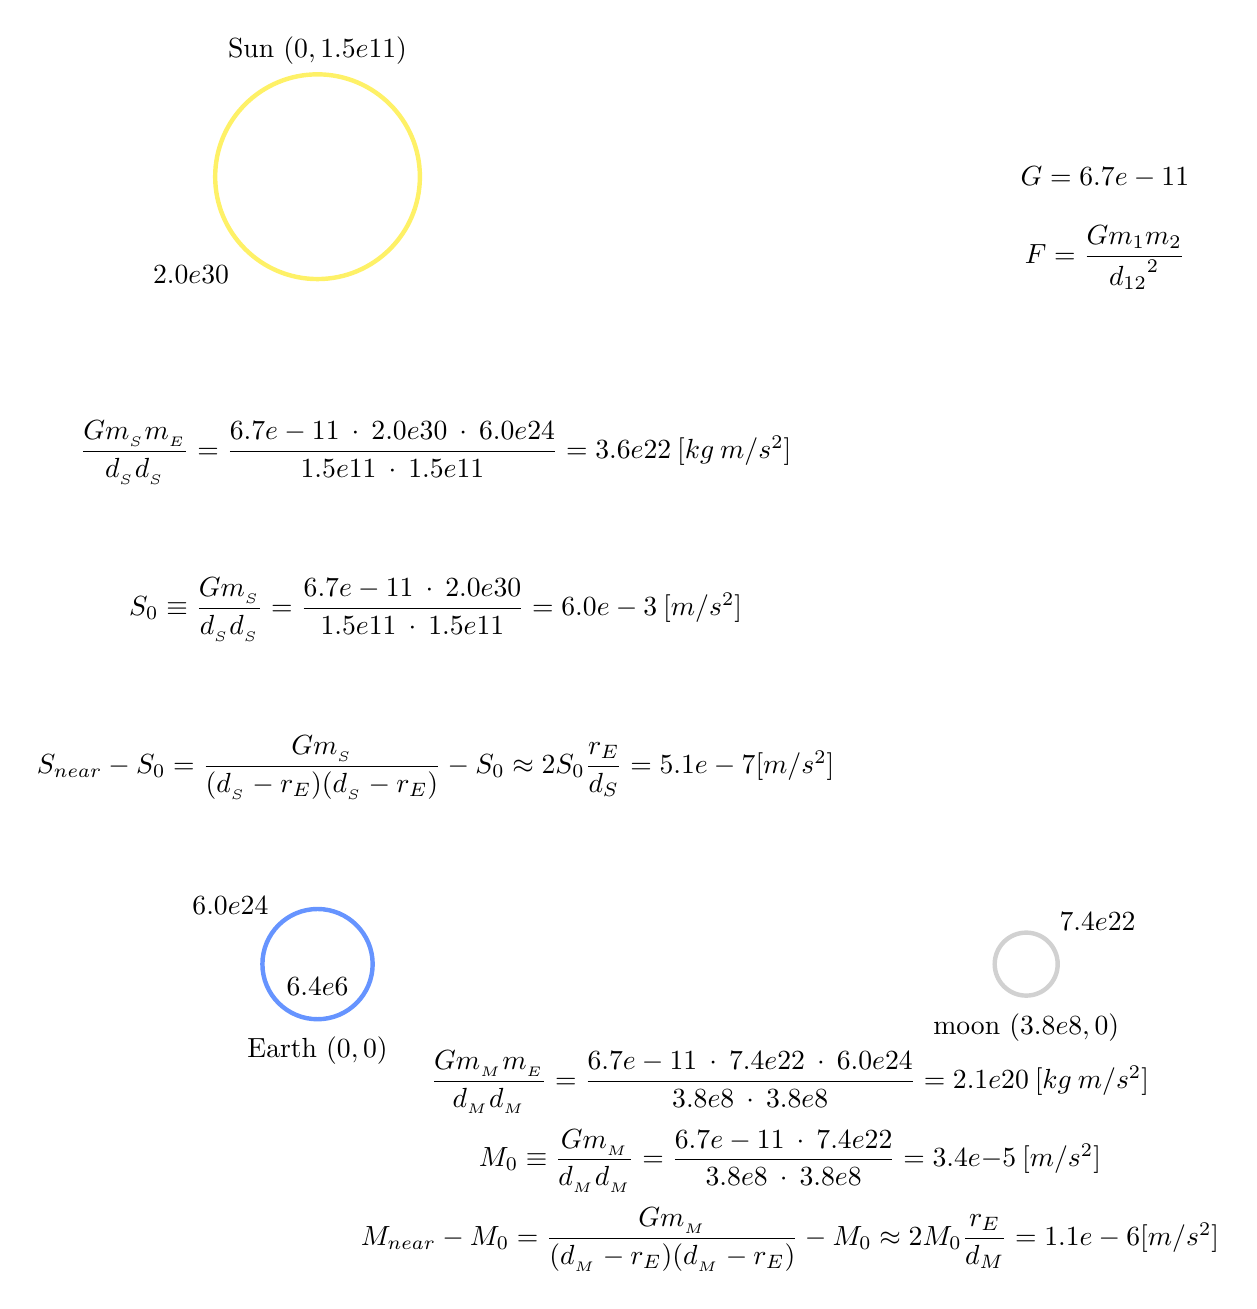
\begin{tikzpicture}
%\begin{tikzpicture}[remember picture, overlay]

    \def\dm{5.0}    % Earth distance from moon along x-axis
    \def\de{4.0}    % Earth distance from moon along x-axis
    \def\ds{0}   % Sun x-coordinate
    \def\dt{7.0}    % Sun y-coordinate

    \coordinate (moon)  at (3,-2);

    \coordinate (Earth) at (-6, -2);

    \coordinate (Sun)   at (-6, 8);

    \coordinate (Ed)   at (4, 8);

    \def\rmoon{0.3}
    \def\rEarth{0.6}
    \def\rSun{1.2}

    \def\eqSz{6}

    % --- SUN ---
    \draw[yellow!90!orange, ultra thick, opacity=0.6] (Sun) circle (\rSun + 0.1);
    \node[above=1.3cm] at (Sun) {Sun $(0, 1.5e11)$};
    \node[below left=1cm] at (Sun) {$2.0e30$};

    % --- EARTH ---
    \draw[blue!70!cyan, ultra thick, opacity=0.6] (Earth) circle (\rEarth + 0.1);
    \node[below=0.8cm] at (Earth) {Earth $(0, 0)$};
    \node[above left=0.5cm] at (Earth) {$6.0e24$};
    \node[below=0.05cm] at (Earth) {$6.4e6$};

    % --- mOON ---
    \draw[black!30!white, ultra thick, opacity=0.6] (moon) circle (\rmoon + 0.1);
    \node[below=0.5cm] at (moon) {moon $(3.8e8,0)$};
    \node[above right=0.3cm] at (moon) {$7.4e22$};

    \node[] at (Ed) {$G=6.7e-11$};
    \node[below=0.5cm] at (Ed) {$F=\dfrac{G m_1 m_2}{{d_{12}}^2}$};

    \node[] at (-4.5,4.5) {$\dfrac{G m_{_S} m_{_E}}{d_{_S} d_{_{S}}}=\dfrac{6.7e-11\hspace{0.75mm}\cdot\hspace{0.75mm}2.0e30\hspace{0.75mm}\cdot\hspace{0.75mm}6.0e24}{1.5e11\hspace{0.75mm}\cdot\hspace{0.75mm}1.5e11}=3.6e22\hspace{0.75mm}[kg\hspace{0.75mm}m/s^2]$};

    \node[] at (-4.5,2.5) {$S_0\equiv\dfrac{G m_{_S}}{d_{_S} d_{_S}}=\dfrac{6.7e-11\hspace{0.75mm}\cdot\hspace{0.75mm}2.0e30}{1.5e11\hspace{0.75mm}\cdot\hspace{0.75mm}1.5e11}=6.0e-3\hspace{0.75mm}[m/s^2]$};

    \node[] at (-4.5,0.5) {$S_{near}-S_0=\dfrac{G m_{_S}}{(d_{_S}-r_E) (d_{_S}-r_E)}-S_0\approx 2 S_0\dfrac{r_E}{d_S}=5.1e-7[m/s^2]$};

    \node[] at (0.0,-3.5) {$\dfrac{G m_{_M} m_{_E}}{d_{_M} d_{_M}}=\dfrac{6.7e-11\hspace{0.75mm}\cdot\hspace{0.75mm}7.4e22\hspace{0.75mm}\cdot\hspace{0.75mm}6.0e24}{3.8e8\hspace{0.75mm}\cdot\hspace{0.75mm}3.8e8}=2.1e20\hspace{0.75mm}[kg\hspace{0.75mm}m/s^2]$};

    \node[] at (0.0,-4.5) {$M_0\equiv\dfrac{G m_{_M}}{d_{_M} d_{_M}}=\dfrac{6.7e-11\hspace{0.75mm}\cdot\hspace{0.75mm}7.4e22}{3.8e8\hspace{0.75mm}\cdot\hspace{0.75mm}3.8e8}=3.4e{-}5\hspace{0.75mm}[m/s^2]$};

    \node[] at (0.0,-5.5) {$M_{near}-M_0=\dfrac{G m_{_M}}{(d_{_M}-r_E) (d_{_M}-r_E)}-M_0\approx2 M_0\dfrac{r_E}{d_M}=1.1e-6[m/s^2]$};

\end{tikzpicture}
\end{document}
